\documentclass{article}

\usepackage{fancyhdr}
\usepackage{extramarks}
\usepackage{amsmath,amssymb,mathrsfs}
\usepackage{amsthm}
\usepackage{amsfonts}
\usepackage{parskip}
\usepackage[version=3]{mhchem} 
\usepackage{fixltx2e}
\usepackage{refcount}
\usepackage{siunitx}
\usepackage{lastpage}
\usepackage{textcomp}
\usepackage{xfrac}
\usepackage{lmodern}
\usepackage{cool}
\usepackage{cancel}
\usepackage{microtype}
\usepackage{gensymb}
\usepackage{enumerate}
\usepackage{float}
\usepackage{bm}
\usepackage{csquotes}
\usepackage{mathtools}
\usepackage{mcode}

\usepackage[hidelinks]{hyperref}

\DeclarePairedDelimiter\bra{\langle}{\rvert}
\DeclarePairedDelimiter\ket{\lvert}{\rangle}
\DeclarePairedDelimiterX\braket[2]{\langle}{\rangle}{#1 \delimsize\vert #2}








%
% Basic Document Settings
%

\topmargin=-0.45in
\evensidemargin=0in
\oddsidemargin=0in
\textwidth=6.5in
\textheight=9.0in
\headsep=0.25in

\linespread{1.1}

\clubpenalty = 10000
\widowpenalty = 10000

\pagestyle{fancy}
\lhead{\hmwkAuthorName}
\chead{\hmwkClass\ \textemdash\ \hmwkTitle}
\rhead{\firstxmark}
\lfoot{\lastxmark}
\cfoot{ASV\twodigits{\thepage}\ of \twodigits{\getpagerefnumber{LastPage}}}

\renewcommand\headrulewidth{0.4pt}
\renewcommand\footrulewidth{0.4pt}

\setlength\parindent{0pt}
\setlength\parskip{1.2ex}





%
% Create Problem Sections
%

\newcommand{\enterProblemHeader}[1]{
    \nobreak\extramarks{}{Problem \arabic{#1} continued on next 
page\ldots}\nobreak{}
    \nobreak\extramarks{Problem \arabic{#1} (continued)}{Problem \arabic{#1} 
continued on next page\ldots}\nobreak{}
}

\newcommand{\exitProblemHeader}[1]{
    \nobreak\extramarks{Problem \arabic{#1} (continued)}{Problem \arabic{#1} 
continued on next page\ldots}\nobreak{}
    \stepcounter{#1}
    \nobreak\extramarks{Problem \arabic{#1}}{}\nobreak{}
    
}

\setcounter{secnumdepth}{0}
\newcounter{partCounter}
\newcounter{homeworkProblemCounter}
\setcounter{homeworkProblemCounter}{1}
\nobreak\extramarks{Problem \arabic{homeworkProblemCounter}}{}\nobreak{}

%
% Homework Problem Environment
%
% This environment takes an optional argument. When given, it will adjust the
% problem counter. This is useful for when the problems given for your
% assignment aren't sequential. See the last 3 problems of this template for an
% example.
%
\newenvironment{homeworkProblem}[1][-1]{
    \ifnum#1>0
	\setcounter{homeworkProblemCounter}{#1}
    \fi
%     \section{Problem \arabic{homeworkProblemCounter}}
    \setcounter{partCounter}{1}
    \enterProblemHeader{homeworkProblemCounter}
}{
    \exitProblemHeader{homeworkProblemCounter}
    \pagebreak

}

%
% Homework Details
%   - Title
%   - Due date
%   - Class
%   - Instructor
%   - Author
%

\newcommand{\hmwkTitle}{Homework\ \# 03}
\newcommand{\hmwkDueDate}{18 October 2016}
\newcommand{\hmwkClass}{NE 255}
\newcommand{\hmwkClassInstructor}{Professor Rachel Slaybaugh}
\newcommand{\hmwkAuthorName}{Andrew S Voyles}

%
% Title Page
%

\title{
%     \vspace{2in}
    \textmd{\textbf{\hmwkClass:\ \hmwkTitle}}\\
    \normalsize\vspace{0.1in}\small{Due\ \hmwkDueDate}\\
    \vspace{0.1in}\large{\textit{\hmwkClassInstructor}}
}

\author{\textbf{\hmwkAuthorName}}
\date{}

\renewcommand{\part}[1]{\textbf{\large Part 
\Alph{partCounter}}\stepcounter{partCounter}\\}

%
% Various Helper Commands
%

% Useful for algorithms
\newcommand{\alg}[1]{\textsc{\bfseries \footnotesize #1}}

% For derivatives
\newcommand{\deriv}[1]{\frac{\mathrm{d}}{\mathrm{d}x} (#1)}

% For partial derivatives
\newcommand{\simplepderiv}[2]{\frac{\partial}{\partial #1} (#2)}

% Integral dx
\newcommand{\dx}{\mathrm{d}x}

% Alias for the Solution section header
\newcommand{\solution}{\textbf{\large Solution}}

% One sentence of lorem ipsum text
\newcommand{\shortlipsum}{Lorem ipsum dolor sit amet, consectetuer adipiscing 
elit.}

% Pad zeroes for footer numbering
\newcommand\twodigits[1]{%
  \ifnum#1<10 0#1\else #1\fi
}

% Consistant figure references
\newcommand{\figref}[1]{Figure~\ref{#1}}

% Define partial derivative alias
\newcommand{\partialder}[2]{\dfrac{\partial #1}{\partial #2}}

% Volume symbol
\newcommand{\volume}{\mathop{\ooalign{\hfil$V$\hfil\cr\kern0.08em--\hfil\cr}}\nolimits}

% Area symbol
\newcommand{\area}{\mathop{\ooalign{\hfil$A$\hfil\cr\kern0.08em--\hfil\cr}}\nolimits}

% Sin and Cos with auto-parentheses 
\newcommand{\sinp}[1]{\sin{\left( #1\right)}}
\newcommand{\cosp}[1]{\cos{\left( #1\right)}}
\newcommand{\expp}[1]{\exp{\left( #1\right)}}
\newcommand{\sinhp}[1]{\sinh{\left( #1\right)}}
\newcommand{\lnp}[1]{\ln{\left( #1\right)}}
\newcommand{\pp}[1]{\left( #1\right)}
\newcommand{\sci}[2]{ #1 \cdot 10^{#2}\ }
\newcommand{\angstrom}{\mbox{\normalfont\AA}}
\newcommand{\norm}[1]{\lVert #1 \rVert}






% math syntax
\newcommand{\nth}{n\ensuremath{^{\text{th}}} }
\newcommand{\ve}[1]{\ensuremath{\mathbf{#1}}}
\newcommand{\Macro}{\ensuremath{\Sigma}}
\newcommand{\rvec}{\ensuremath{\vec{r}}}
\newcommand{\xvec}{\ensuremath{\vec{x}}}
\newcommand{\omvec}{\ensuremath{\hat{\Omega}}}
\newcommand{\vOmega}{\ensuremath{\hat{\Omega}}}


% Make vectors use boldface
\renewcommand{\vec}[1]{\mathbf{#1}}


% Consistant matrix notation
\newcommand{\matr}[1]{\mathbf{#1}} % undergraduate algebra version
% \newcommand{\matr}[1]{#1}          % pure math version
% \newcommand{\matr}[1]{\boldsymbol{#1}}     % ISO complying version


\makeatletter
% Make common definition of mean
\newcommand*\mean[1]{\overline{#1\raisebox{3mm}{}}}

\makeatother






\begin{document}

\maketitle
\thispagestyle{fancy}





\section{Problem 1}

\begin{homeworkProblem}

 (20 points)  Derive the 1st order form of $SP_5$ with isotropic source and vacuum boundary
conditions.




\subsection{Solution}
    
 XXXXXXXXXXXXXXXXXX
    

\end{homeworkProblem}


\section{Problem 2}

\begin{homeworkProblem}

Consider the integral

\begin{equation}
\int_{4\pi} d\omvec \left|\omvec\right|
\end{equation}

The LQ$_N$ quadrature set is given in \autoref{fig:LQquad}. Recall that $\mu_i = \eta_i = \xi_i$ for a given level, $i$.

\begin{figure}[H]
 \centering
 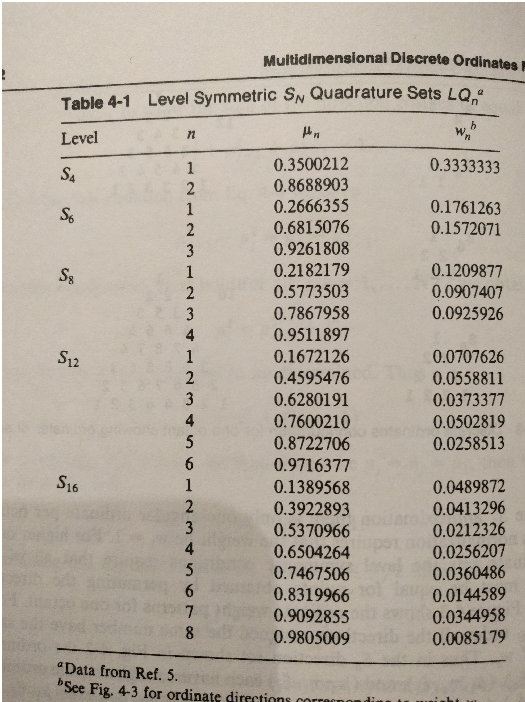
\includegraphics{./homework3-cropped.pdf}
 % homework3-cropped.pdf: 252x337 pixel, 72dpi, 8.89x11.89 cm, bb=0 0 252 337
 \caption{LQ$_n$ quadrature}
 \label{fig:LQquad}
\end{figure}


\begin{enumerate}[(a)] 

\item  (5 points)  Use the $S_4$ LQ$_N$ quadrature set to execute this integral.





\subsection{Solution}
    
  XXXXXXXXXXXXXXXXXXXXXX
 
   
\item    (10 points) Repeat it with $S_6$. What do you observe?




\subsection{Solution}
    
  XXXXXXXXXXXXXXXXXX
   
   \item (10 points) Write a short code to execute this integration (and higher orders if
you'd like). Try a few different functions. Turn in the code and the evaluation of
these functions. Include comments on what you observe.



\subsection{Solution}
    
  XXXXXXXXXXXXXXXXX


\end{enumerate}

\end{homeworkProblem}


\section{Problem 3}

\begin{homeworkProblem}




\begin{enumerate}[(a)] 

\item (5 points) Briefly compare the diffusion equation, deterministic methods, and monte
carlo methods in terms of complexity, accuracy, run time, and range of applicability.




\subsection{Solution}

XXXXXXXXXXXXXXXXXXXXXXXX
 
   
\item  (5 points) Given what you've learned about deterministic methods so far, discuss
strengths and weaknesses.




\subsection{Solution}

   XXXXXXXXXXXXXXXXXXXXXXXXXXXXx
   

\end{enumerate}

\end{homeworkProblem}



\section{Problem 4}

\begin{homeworkProblem}

Write a function that generates the associated Legendre Polynomials:

\begin{equation}
P_\ell^m\pp{x} = \dfrac{\pp{-1}^m}{2^\ell \ell!} \pp{1-x^2}^{m/2} \dfrac{d^{\ell+m}}{dx^{\ell+m}} \pp{x^2-1}^\ell
\end{equation}

Use this function in a function that generates spherical harmonics:

\begin{equation}
Y_{\ell m} \pp{\theta,\phi} = \pp{-1}^m \sqrt{\dfrac{2\ell+m}{4\pi} \dfrac{\pp{\ell-m}!}{\pp{\ell+m}!}} P_{\ell m}\pp{\cosp{\theta}} e^{i m \phi} 
\end{equation}



\begin{enumerate}[(a)] 

\item  (30 points) Generate and plot the following $\ell$ = 0, 1, 2 for $-\ell \leq m \leq \ell$ (recall we
can relate the negate $m$ to positive $m$ values). You will need to discretize $\theta$ and $\phi$
fairly finely (I suggest 30 increments in each to start so you get a real sense of the
shape of the harmonics).




\subsection{Solution}
    
XXXXXXXXXXXXXXXXXX

   
   
\item (20 points)    Now, we will approximate the external source. Using the $S_4$ quadrature
to do the integrations and $q_e$ = 1 for all angles: use the equations for external source
we developed in class (eqns. 19-21), calculate the external source for $\ell$ = 0, 1, 2.


\subsection{Solution}
    
   XXXXXXXXXXXXXXXXXXXXX
   
\begin{figure}[H]
\centering
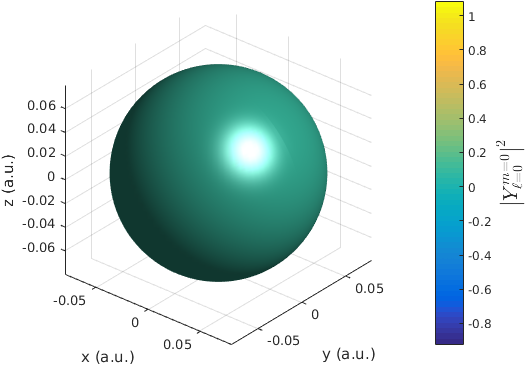
\includegraphics{./Y00.png}
% hw02_03a.pdf: 204x92 pixel, 72dpi, 7.20x3.25 cm, bb=0 0 204 92
 \caption{Y00}
\label{fig:Y00}
\end{figure}

\begin{figure}[H]
\centering
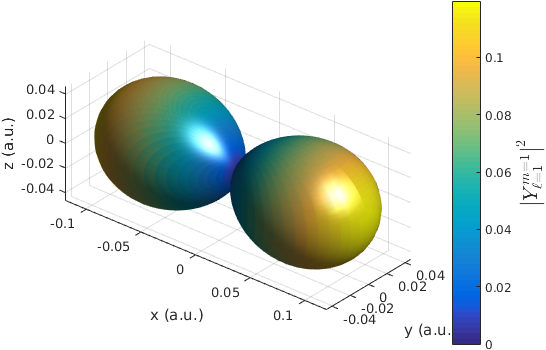
\includegraphics{./Y11.png}
% hw02_03a.pdf: 204x92 pixel, 72dpi, 7.20x3.25 cm, bb=0 0 204 92
 \caption{Y11}
\label{fig:Y11}
\end{figure}

\begin{figure}[H]
\centering
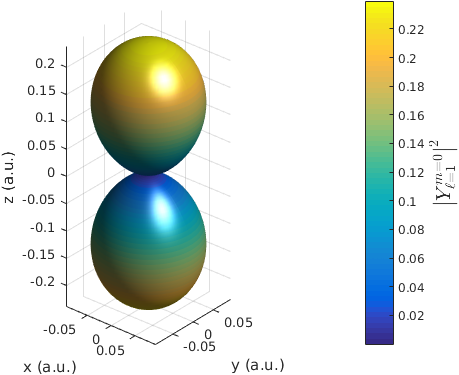
\includegraphics{./Y10.png}
% hw02_03a.pdf: 204x92 pixel, 72dpi, 7.20x3.25 cm, bb=0 0 204 92
 \caption{Y10}
\label{fig:Y10}
\end{figure}



\begin{figure}[H]
\centering
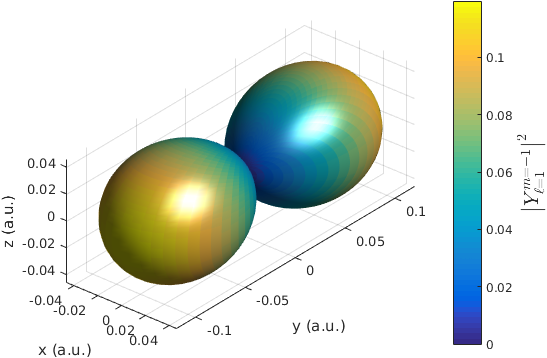
\includegraphics{./Y1-1.png}
% hw02_03a.pdf: 204x92 pixel, 72dpi, 7.20x3.25 cm, bb=0 0 204 92
 \caption{Y1-1}
\label{fig:Y1-1}
\end{figure}

\begin{figure}[H]
\centering
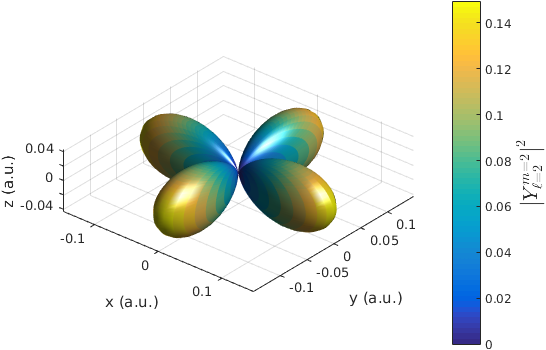
\includegraphics{./Y22.png}
% hw02_03a.pdf: 204x92 pixel, 72dpi, 7.20x3.25 cm, bb=0 0 204 92
 \caption{Y22}
\label{fig:Y22}
\end{figure}

\begin{figure}[H]
\centering
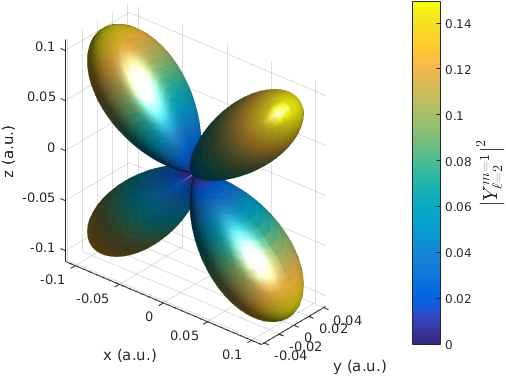
\includegraphics{./Y21.png}
% hw02_03a.pdf: 204x92 pixel, 72dpi, 7.20x3.25 cm, bb=0 0 204 92
 \caption{Y21}
\label{fig:Y21}
\end{figure}

\begin{figure}[H]
\centering
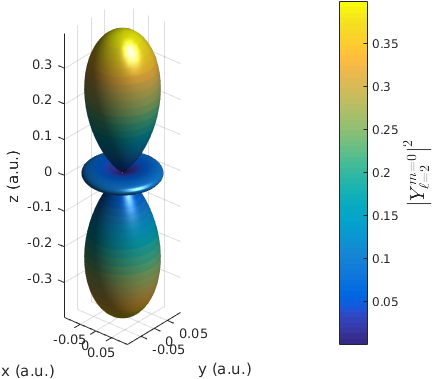
\includegraphics{./Y20.png}
% hw02_03a.pdf: 204x92 pixel, 72dpi, 7.20x3.25 cm, bb=0 0 204 92
 \caption{Y20}
\label{fig:Y20}
\end{figure}

\begin{figure}[H]
\centering
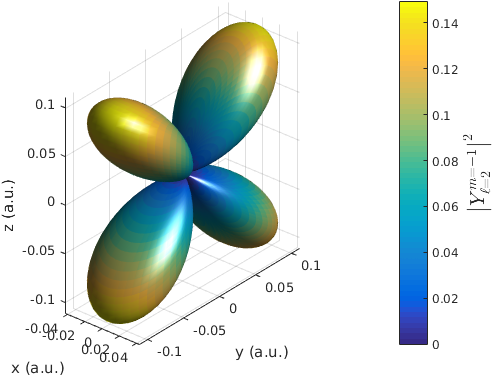
\includegraphics{./Y2-1.png}
% hw02_03a.pdf: 204x92 pixel, 72dpi, 7.20x3.25 cm, bb=0 0 204 92
 \caption{Y2-1}
\label{fig:Y2-1}
\end{figure}

\begin{figure}[H]
\centering
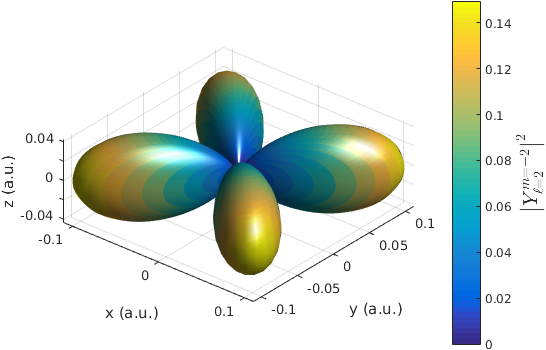
\includegraphics{./Y2-2.png}
% hw02_03a.pdf: 204x92 pixel, 72dpi, 7.20x3.25 cm, bb=0 0 204 92
 \caption{Y2-2}
\label{fig:Y2-2}
\end{figure}




    \end{enumerate}
    
 

\end{homeworkProblem}




\section{Problem 5}

\begin{homeworkProblem}

(5 points) What are the major nuclear data libraries and which countries manage them?


\subsection{Solution}
    
  A large number of these nuclear data libraries currently exist, each of which serve a specific purpose within the global nuclear data community.
  
  
  At the most fundamental level, nuclear data consists of the various input parameters used in structure and reaction evaluation codes. Since computational tools are currently incapable of describing single nuclei at the microscopic level of a many-nucleon wavefunction, bulk nuclear properties and data are instead modeled using a parameterized model of spherical or deformed nuclei, whose parameters are determined via fitting to experimental measurements of these properties. Once best-fit input parameters are determined, they can be used as predictive and evaluation tools. The primary fundamental libraries are the Reference Input Parameter Library (RIPL), which collects nuclear masses, discrete nuclear levels, neutron resonances, nuclear optical model parameters, nuclear level densities, and photon resonances, and  the Evaluated Gamma-ray Activation File (EGAF), which collects nuclear level densities, level parities, and radiative strength functions. Both of these libraries are maintained by the IAEA.
  
  
  Stepping up one level of application are the experimental libraries, which act as a stepping stone between experimental publications and the evaluated libraries. When researchers publish experimental measurements of nuclear data, the authors are able to compile their results into an experimental library. These libraries provide \enquote{bleeding-edge} nuclear data measurements for the nuclear community, but also serve as the inputs used in the periodic evaluation updates of the various evaluated data libraries. The experimental libraries include the Experimental Unevaluated Nuclear Data List (XUNDL), which collects experimental nuclear structure and decay data, and the Experimental Nuclear Reaction Data Library (EXFOR/CSISRS), which collects experimental nuclear reaction data. Both of these libraries are maintained by the US Nuclear Data Program, under the auspices of the National Nuclear Data Center (NNDC).
  
  
  The next step in the nuclear data community is the evaluation process, which collects the compiled experimental data in XUNDL/EXFOR and assigns recommended values for the data. This involves a review of the experimental methods used in each publication, as well as using the different evaluation codes to verify that the recommended values agree with nuclear theoretical models, as well as to weed out any poorly-designed experiments which may have produced inaccurate data. These evaluations thus produce the \enquote{best} statistically recommended values for all measured nuclear data, as well as statistical covariances in measurement uncertainties. These libraries include  the Evaluated Nuclear Structure Data File (ENSDF), which is a nuclear structure and decay library evaluated from the XUNDL library using the  EMPIRE\footnote{\url{  http://www.nndc.bnl.gov/empire/}} evaluation code, and the Evaluated Nuclear Data File (ENDF), a nuclear reaction data library evaluated from the EXFOR library using the  EMPIRE evaluation code. Both of these libraries are maintained by the US Nuclear Data Program, under the auspices of the National Nuclear Data Center (NNDC). Other evaluated libraries include:
  
  \begin{itemize}
    

  
  \item the TALYS-based Evaluated Nuclear Data Library (TENDL), an IAEA-maintained nuclear reaction data library evaluated directly from experimental publications using the   TALYS\footnote{\url{http://www.talys.eu/}}  evaluation code, 
  
  \item the  Joint Evaluated Fission and Fusion File (JEFF), an evaluated library of nuclear reactions, decay data, and fission yields maintained by the Nuclear Energy Agency Data Bank member countries\footnote{Austria,	Germany	,	Mexico	,	Slovak Republic,	Belgium	,	Greece	,	Netherlands	,	Slovenia,	Czech Republic	 ,	Hungary	,	Norway	,	Spain
,	Denmark	,	Italy	,	Poland	,Sweden
,	Finland	,	Japan	,	Portugal	,	Switzerland
,	France	,Republic of Korea ,	Russia	,	Turkey,	 	 	United Kingdom}, which is evaluated using the TALYS and ALICE\footnote{\url{https://rsicc.ornl.gov/codes/psr/psr1/psr-146.html}} codes,


  \item the Japanese Evaluated Nuclear Data Library (JENDL), an evaluated  neutron reaction data library, maintained by Japan,
  
  \item the Bruyeres-le-chatel Discrete Level Library (BRC), a defense-oriented evaluated neutron data library, maintained by the French Alternative Energies and Atomic Energy Commission (CEA) ,
  
  \item the Karlsruhe Nuclear Data Library (KEDAK), a primarily low-energy neutron resonance evaluated library. This library was maintained by Germany, but has since been absorbed into JEFF and WLUP (see below).
  
    \end{itemize}

  
  All of the evaluated libraries listed up to this point are compilations of fundamental nuclear parameters: nuclear levels, widths, lifetimes, transition elements, and the like, leading up to cross-sections as the highest-level piece of data. While these fundamental parameters are important, they are often too low-level for many applications and calculations. As a result, there exist many application-specific libraries, which report the relevant pieces of nuclear data for specific scenarios, in units convenient to those applications. While there are a multitude of these libraries, two important ones are addressed here.  Nuclear Structure and Decay Data (NuDat) is a compiled library which reads from ENSDF, and reports all of the decay radiation (with relative intensities, branching ratios, coincidence peaks, and level transition elements), along with basic properties of radioactive nuclei: half-lives, Q-values, decay schemes, nucleon separation energies, and the like. These are all presented in a simple and user-friendly web format useful for calculations, and are maintained by the NNDC.  The Medical Internal Radiation Dose (MIRD) library is another nuclear decay library maintained by the NNDC, which lists NuDat decay data, in terms of the dose associated with various decay radiations. These are useful for dose planning, radiation shielding calculations, and other situations where human dose is considered. The International Reactor Dosimetry and Fusion File (IRDFF) is an IAEA-maintained library of medical isotope production cross sections and excitation functions, charged particle beam monitor reaction data, and dosimetry standards. The WIMS[Winfrith Improved Multigroup Scheme-D] Library Update Project (WLUP) is an IAEA-maintained library of neutron multigroup evaluated cross sections, and is one the only open-source libraries of this data, which is often commercial / closed-source, due to their value in reactor lattice transport calculations.
  
 

\end{homeworkProblem}



\end{document}
